\documentclass[aspectratio=169,11pt]{beamer}
% ==========================================================================
%  KSA lecture-slide theme  =  stock beamer "Boadilla"  +  KSA colour theme
%  brand colours sampled from the official KSA symbol mark:
%    Deep Prussian Blue  #2E3192   (지성 - intellect)
%    Golden Gray         #D6CBB1   (감성 - sensibility)
%  Engine: XeLaTeX.  Usage:
%    \documentclass[aspectratio=169,11pt]{beamer}
%    \input{../../theme/ksa-theme.tex}
%  Each deck lives in its own slides/kor/<deck>/ folder together with its
%  own images; ../../figs/ is kept only as a fallback for the shared cache.
% ==========================================================================

\usepackage{fontspec}
\usepackage{amsmath,amssymb}
\usepackage{graphicx}
\graphicspath{{figs/}{./}{../../../figs/}}
\usepackage{booktabs}
\usepackage{listings}
\usepackage{varwidth}

% ---- fonts (no ctex/xeCJK on this box -> fontspec drives CJK directly) -----
\defaultfontfeatures{Ligatures=TeX}
\setmainfont{Noto Sans CJK KR}
\setsansfont{Noto Sans CJK KR}
\setmonofont{Noto Sans Mono CJK KR}[Scale=0.92]

% ---- base theme: stock Boadilla ------------------------------------------
\usetheme{Boadilla}
\usefonttheme{professionalfonts}
\setbeamertemplate{navigation symbols}{}

% ---- KSA colour theme (recolour the stock theme) --------------------------
\definecolor{ksablue}{HTML}{2E3192}
\definecolor{ksabluedk}{HTML}{20226A}
\definecolor{ksagold}{HTML}{D6CBB1}
\definecolor{ksagolddk}{HTML}{A9976B}
\definecolor{ksared}{HTML}{C0392B}
\definecolor{ksagray}{HTML}{5B5B5B}

\setbeamercolor{structure}{fg=ksablue}
\setbeamercolor{alerted text}{fg=ksared}

\setbeamercolor{palette primary}{fg=white,           bg=ksablue}
\setbeamercolor{palette secondary}{fg=white,         bg=ksablue!85!black}
\setbeamercolor{palette tertiary}{fg=white,          bg=ksabluedk}
\setbeamercolor{titlelike}{fg=ksablue}
\setbeamercolor{frametitle}{fg=ksablue,bg=}
\setbeamercolor{title}{fg=ksablue}
\setbeamercolor{author}{fg=ksagray}
\setbeamercolor{institute}{fg=ksagray}
\setbeamercolor{block title}{fg=white,bg=ksablue}
\setbeamercolor{block body}{fg=black!85,bg=ksablue!6}
\setbeamercolor{item}{fg=ksablue}
\setbeamercolor{section in toc}{fg=black!85}

\setbeamerfont{frametitle}{series=\bfseries}
\setbeamerfont{title}{series=\bfseries}

% ---- footline:  KSA mark | "Made by ..." | n / N   (matches reference) ----
\newcommand{\ksacredit}{}
\setbeamertemplate{footline}{%
  \hbox{%
    \begin{beamercolorbox}[wd=.18\paperwidth,ht=2.6ex,dp=1.5ex,leftskip=1.1em]{}%
      \raisebox{-0.35ex}{\includegraphics[height=2.0ex]{ksa-logo.png}}%
    \end{beamercolorbox}%
    \begin{beamercolorbox}[wd=.64\paperwidth,ht=2.6ex,dp=1.5ex,center]{}%
      {\scriptsize\color{ksagray}\ksacredit}%
    \end{beamercolorbox}%
    \begin{beamercolorbox}[wd=.18\paperwidth,ht=2.6ex,dp=1.5ex,rightskip=1.1em]{}%
      \hfill{\scriptsize\color{ksablue}\insertframenumber\,/\,\inserttotalframenumber}%
    \end{beamercolorbox}%
  }%
  \vskip2pt
}

% ---- section divider: stock \sectionpage, KSA-coloured -------------------
\setbeamertemplate{section page}{%
  \begingroup\centering
    {\color{ksagolddk}\rule{0.16\paperwidth}{1pt}}\par\vskip1.0em
    {\usebeamerfont{title}\color{ksablue}\insertsectionhead\par}\vskip1.0em
    {\color{ksagolddk}\rule{0.16\paperwidth}{1pt}}\par
  \endgroup
}
\AtBeginSection[]{\begin{frame}[plain,noframenumbering]\vfill\sectionpage\vfill\end{frame}}

% ---- code listings ------------------------------------------------------------
\lstdefinestyle{ksa}{%
  basicstyle=\ttfamily\scriptsize,
  keywordstyle=\color{ksablue}\bfseries,
  commentstyle=\color{ksagray}\itshape,
  stringstyle=\color{ksagolddk},
  numberstyle=\tiny\color{ksagray},
  backgroundcolor=\color{ksablue!6},
  frame=leftline, framerule=1.4pt, rulecolor=\color{ksablue},
  xleftmargin=1em, aboveskip=0.8em, belowskip=0.4em,
  showstringspaces=false, breaklines=true, language=Python,
}
\lstset{style=ksa}

% ---- handy macros -----------------------------------------------------------
\newcommand{\kb}[1]{\textbf{\color{ksablue}#1}}   % blue keyword
\newcommand{\kq}[1]{\textbf{\color{ksared}#1}}    % red key-question

\setbeamerfont{title}{series=\bfseries,size=\fontsize{24}{30}\selectfont}
\setbeamerfont{subtitle}{series=\bfseries,size=\fontsize{14}{18}\selectfont}
\setbeamerfont{author}{size=\normalsize}
\setbeamerfont{institute}{size=\small}
\graphicspath{{figs/}{../../../../assets/}}
\makeatletter
\newcommand{\markpage}[1]{\protected@write\@auxout{}{\string\newlabel{#1}{{\the\c@framenumber}{}}}\hypertarget{#1}{}}
\newcommand{\pref}[1]{\hyperlink{#1}{\textcolor{ksagolddk}{(p.\ref{#1})}}}
\makeatother
% IBM AML HI-Small 숫자 (exp_aml.py → assets/aml.json 에서 옮겨 적었고 data.py 가 같은지 확인한다)
\newcommand{\amlN}{5{,}078{,}345}          % 거래 수
\newcommand{\amlPos}{5{,}177}        % 세탁 거래 수
\newcommand{\amlRate}{0.10}       % 세탁 비율 (%)
\newcommand{\amlAccZero}{99.90}    % 전부 '정상' 정확도 (%)
\newcommand{\amlFmt}{ACH (자동 이체)}        % 규칙에 쓴 결제 형식
\newcommand{\amlAccRule}{88.24}    % 규칙 정확도 (%)
\newcommand{\amlTP}{4{,}483}\newcommand{\amlFP}{596{,}314}\newcommand{\amlFN}{694}
\newcommand{\amlPrec}{0.75}       % 규칙 정밀도 (%)
\newcommand{\amlRec}{86.6}        % 규칙 재현율 (%)
\newcommand{\amlAcct}{496{,}999}       % 보낸 계좌 수
\newcommand{\amlAcctPos}{3{,}376}    % 세탁 거래를 보낸 계좌 수
\newcommand{\amlAcctRate}{0.68}   % 계좌 단위 세탁 비율 (%)
\newcommand{\amlDays}{18일 (2022-09-01 $\sim$ 09-18)}       % 기간
\newcommand{\amlRowA}{2022/09/01 00:20 & 10, 8000EBD30 & 10, 8000EBD30 & 3,697.34 & US Dollar & Reinvestment & 0}   % 실제 첫 줄
\newcommand{\amlRowB}{2022/09/01 00:20 & 3208, 8000F4580 & 1, 8000F5340 & 0.01 & US Dollar & Cheque & 0}

\renewcommand{\ksacredit}{Machine Learning 1 \,\textperiodcentered\, 문제 정형화와 평가지표}
\title{문제 정형화와 평가지표}
\subtitle{Problem Formulation · Metrics · Baselines --- 무엇을 맞히고, 어떻게 채점하나}
\author{Machine Learning 1}
\institute{한국과학영재학교 (KSA)}
\date{}
\begin{document}
\begin{frame}[plain,noframenumbering]\titlepage\end{frame}

% --- 오늘의 질문
\begin{frame}{오늘의 질문}
\vfill
\centering
{\Large 자금세탁 거래를 찾는 모델을 만들었다.}\vskip0.8em
{\fontsize{40}{48}\selectfont\textbf{정확도 \kb{\amlAccZero\%}}}\vskip1em
{\Large 좋은 모델일까?}\vskip1.4em
{\small IBM AML 데이터 (합성 은행 거래 \amlN 건)}
\vfill
\note{은행 거래 기록에서 자금세탁 거래를 찾는 모델을 만들었다고 해 봅시다. 정확도가 \amlAccZero 퍼센트입니다. 좋은 모델일까요? 답부터 말하면, 이 모델은 아무것도 하지 않습니다. 모든 거래에 정상이라고만 답합니다. 세탁 거래가 전체의 \amlRate 퍼센트뿐이라서, 그것만으로도 이 점수가 나옵니다. 문제를 어떻게 정의하고 무엇으로 채점하느냐를 정하지 않으면, 숫자가 아무리 좋아도 의미가 없습니다. 오늘은 모델을 만들기 전에 할 일, 문제를 정형화하는 법을 배웁니다.}
\end{frame}

% --- 다섯 칸
\begin{frame}{머신러닝 문제 = 다섯 칸 채우기}
\markpage{five}
\vfill
\centering
{\large
\begin{tabular}{rll}
\kb{①} & \textbf{한 행은 무엇?} & 예시 하나의 단위: 와인 한 병, 거래 한 건, 계좌 하나\\[0.5em]
\kb{②} & \textbf{입력 $X$} & 예측할 때 \textbf{알 수 있는} 것만\\[0.5em]
\kb{③} & \textbf{출력 $y$} & 맞히려는 것: 품종? 도수? 세탁 여부? 3D 구조?\\[0.5em]
\kb{④} & \textbf{평가지표} & 무엇으로 채점하나: 정확도, MAE, 정밀도 · 재현율 \ldots\\[0.5em]
\kb{⑤} & \textbf{기준선} & 머리 안 쓰는 답의 점수: 가장 흔한 답, 평균, 지난달 그대로
\end{tabular}}\vskip1.2em
{\large 다섯 칸이 정해져야 \kq{``잘했다''를 말할 수 있다}}
\vfill
\note{머신러닝 문제를 정한다는 건 다섯 칸을 채우는 일입니다. 첫째, 한 행, 즉 예시 하나가 무엇인지. 와인 한 병인지, 거래 한 건인지, 계좌 하나인지. 둘째, 입력. 예측하는 순간에 실제로 알 수 있는 것만 넣어야 합니다. 셋째, 출력, 맞히려는 것. 넷째, 평가지표, 무엇으로 채점할지. 다섯째, 기준선, 머리를 전혀 안 쓴 답이 몇 점인지. 이 다섯 칸이 정해져야 우리 모델이 잘했다, 못했다를 말할 수 있습니다.}
\end{frame}

% --- 문제 종류
\begin{frame}{출력 $y$ 의 모양이 문제의 종류를 정한다}
\vfill
\centering
{\large
\begin{tabular}{lll}
\textbf{출력 $y$} & \textbf{문제 종류} & \textbf{예}\\[0.2em]\hline\\[-0.6em]
범주 하나 & \kb{분류} (classification) & 와인 품종 (3개 중 하나), 세탁인가 (예/아니오)\\[0.5em]
숫자 하나 & \kb{회귀} (regression) & 알코올 도수, 다음 달 항공 승객 수\\[0.5em]
숫자 여러 개 & 위치 예측 & 사진 속 고양이의 위치 (상자 좌표 4개)\\[0.5em]
글 · 그림 & 생성 & 다음 단어, 그림 (14주차 이후)
\end{tabular}}\vskip1.2em
{\large 같은 데이터라도 \kq{$y$ 를 무엇으로 정하느냐}에 따라 다른 문제가 된다}
\vfill
\note{출력의 모양이 문제의 종류를 정합니다. 범주 중 하나를 고르면 분류, 숫자 하나를 맞히면 회귀입니다. 사진 속 물체의 위치처럼 숫자 여러 개를 한꺼번에 맞히는 문제도 있고, 글이나 그림을 만드는 생성 문제도 있습니다. 중요한 건, 데이터가 문제를 정하는 게 아니라 우리가 y를 무엇으로 정하느냐가 문제를 정한다는 겁니다. 실제로 해 봅시다.}
\end{frame}

% --- 와인 두 문제
\begin{frame}{같은 와인 178병, 두 문제}
\vfill
\centering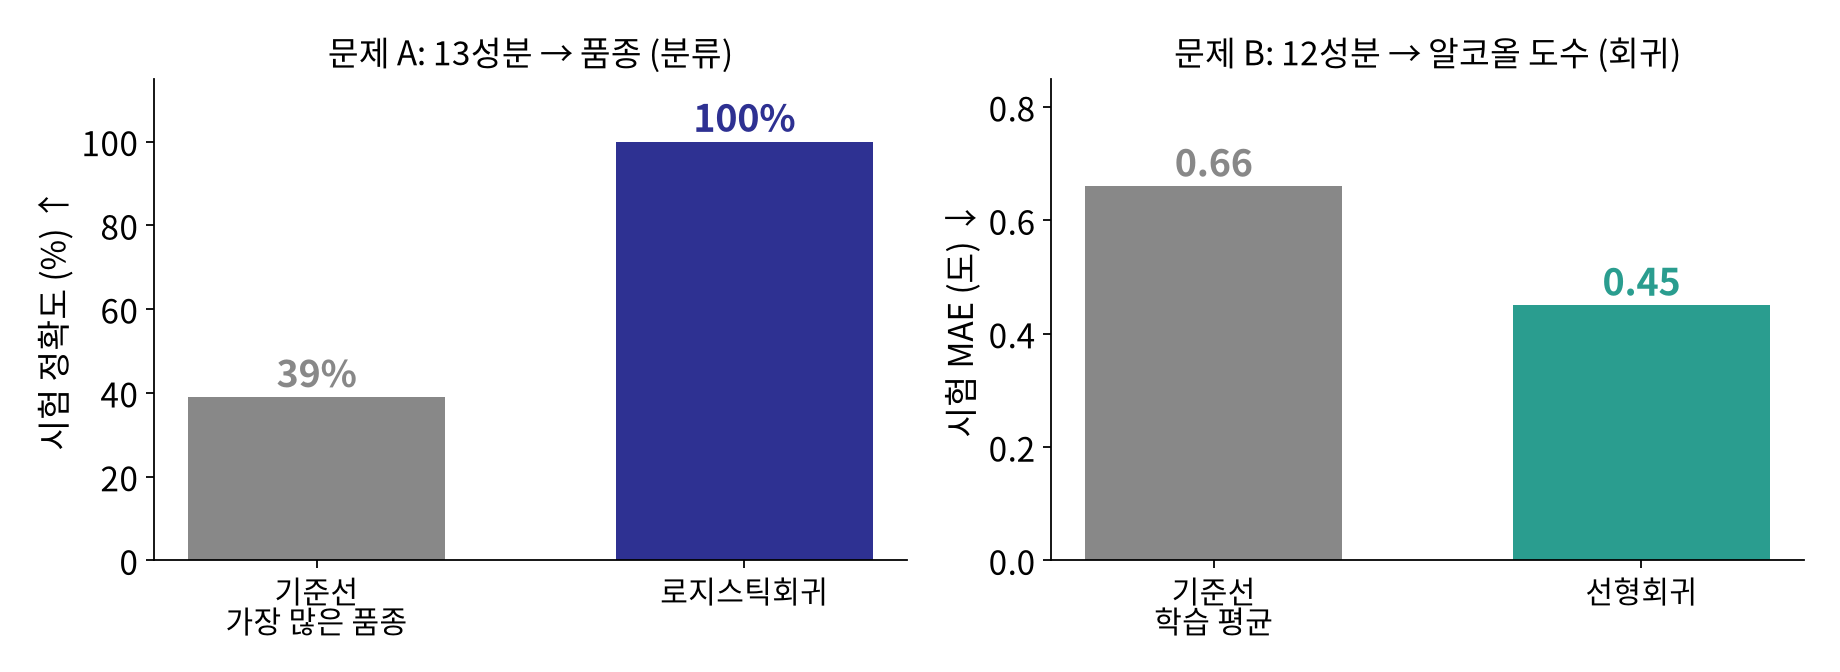
\includegraphics[width=0.84\linewidth]{pf_wine.png}\par\vskip0.3em
{\large 문제 A: $y$ = 품종 $\to$ \kb{정확도} \qquad 문제 B: $y$ = 알코올 도수 (11.03 $\sim$ 14.83도) $\to$ \kb{MAE}}\\[0.3em]
{\scriptsize 학습 70\% · 시험 30\% (54병), 표준화 + 로지스틱회귀 / 선형회귀. 문제 B 의 입력에는 알코올을 넣지 않는다 (답을 입력에 넣으면 안 된다)}
\vfill
\note{지난 시간 그 와인 데이터입니다. 문제 A는 성분 13가지로 품종을 맞히는 분류입니다. 채점은 정확도, 시험 54병 중 몇 병을 맞혔나. 로지스틱회귀가 100퍼센트를 맞힙니다. 문제 B는 같은 데이터에서 알코올 도수를 맞히는 회귀입니다. 이때 입력에서 알코올은 빼야 합니다. 답을 입력에 넣으면 당연히 맞히겠죠. 채점은 MAE, 평균적으로 몇 도 틀렸나입니다. 선형회귀가 0.45도, 기준선이 0.66도입니다. 같은 데이터, 다른 y, 다른 지표입니다. 각 그래프의 회색 막대가 기준선인데, 이건 조금 뒤에 다시 봅니다.}
\end{frame}

% --- 회귀 지표
\begin{frame}{회귀의 채점: MAE 와 RMSE}
\vfill
\centering
{\Large
\[ \text{MAE} = \frac{1}{n}\sum_{i=1}^{n} |\,y_i - \hat y_i\,| \qquad\qquad \text{RMSE} = \sqrt{\frac{1}{n}\sum_{i=1}^{n} (y_i - \hat y_i)^2} \]}\vskip0.6em
{\large $y_i$ = 정답, \quad $\hat y_i$ = 예측, \quad 둘 다 \kb{$y$ 와 같은 단위} (도, 명, cm)}\vskip1em
{\large 오차 \texttt{[1, 1, 1, 9]}: \quad MAE $= \dfrac{1+1+1+9}{4} = \kb{3}$ \qquad RMSE $= \sqrt{\dfrac{1+1+1+81}{4}} = \sqrt{21} = \kq{4.58}$}\vskip1em
{\small RMSE 는 제곱하니까 \textbf{크게 틀린 하나}에 더 큰 벌을 준다. 무엇이 더 나쁜지에 따라 고른다}
\vfill
\note{회귀는 얼마나 틀렸는지를 잽니다. MAE는 오차의 절댓값 평균, RMSE는 오차를 제곱해 평균 내고 루트를 씌운 겁니다. 둘 다 y와 단위가 같아서 해석하기 쉽습니다. 오차가 1, 1, 1, 9인 예를 보면 MAE는 3, RMSE는 루트 21, 4.58입니다. 9짜리 오차 하나가 제곱되면서 RMSE를 끌어올렸습니다. 작게 여러 번 틀리는 것보다 한 번 크게 틀리는 게 더 나쁜 문제, 예를 들어 다리 하중 예측이라면 RMSE를 씁니다.}
\end{frame}

% --- 기준선
\begin{frame}{기준선: 머리를 안 쓴 답은 몇 점인가}
\markpage{baseline}
\vfill
\centering
{\large
\begin{tabular}{lll}
\textbf{문제} & \textbf{기준선} & \textbf{점수}\\[0.2em]\hline\\[-0.6em]
와인 품종 (분류) & 늘 가장 많은 품종 (71병짜리) 이라고 답 & 정확도 \kq{39\%}\\[0.5em]
알코올 도수 (회귀) & 늘 학습 데이터의 평균 도수라고 답 & MAE \kq{0.66도}\\[0.5em]
항공 승객 (시계열) & 늘 지난달 승객 수라고 답 & MAE \kq{44천 명}\\[0.5em]
자금세탁 (분류) & 늘 ``정상''이라고 답 & 정확도 \kq{\amlAccZero\%}
\end{tabular}}\vskip1.2em
{\large 모델 점수는 \kb{기준선과 비교}해서 읽는다}
\vfill
\note{기준선은 머리를 전혀 쓰지 않은 답입니다. 분류면 늘 가장 흔한 답, 회귀면 늘 평균, 시계열이면 늘 지난달 값. 와인 품종의 기준선은 39퍼센트라서 100퍼센트는 대단한 점수입니다. 반대로 자금세탁은 기준선이 \amlAccZero 퍼센트라서, 99퍼센트 모델은 기준선보다 못한 모델입니다. 같은 99퍼센트라도 기준선에 따라 의미가 정반대입니다.}
\end{frame}

% --- 항공 승객 기준선
\begin{frame}{모델이 기준선보다 못할 수도 있다}
\vfill
\centering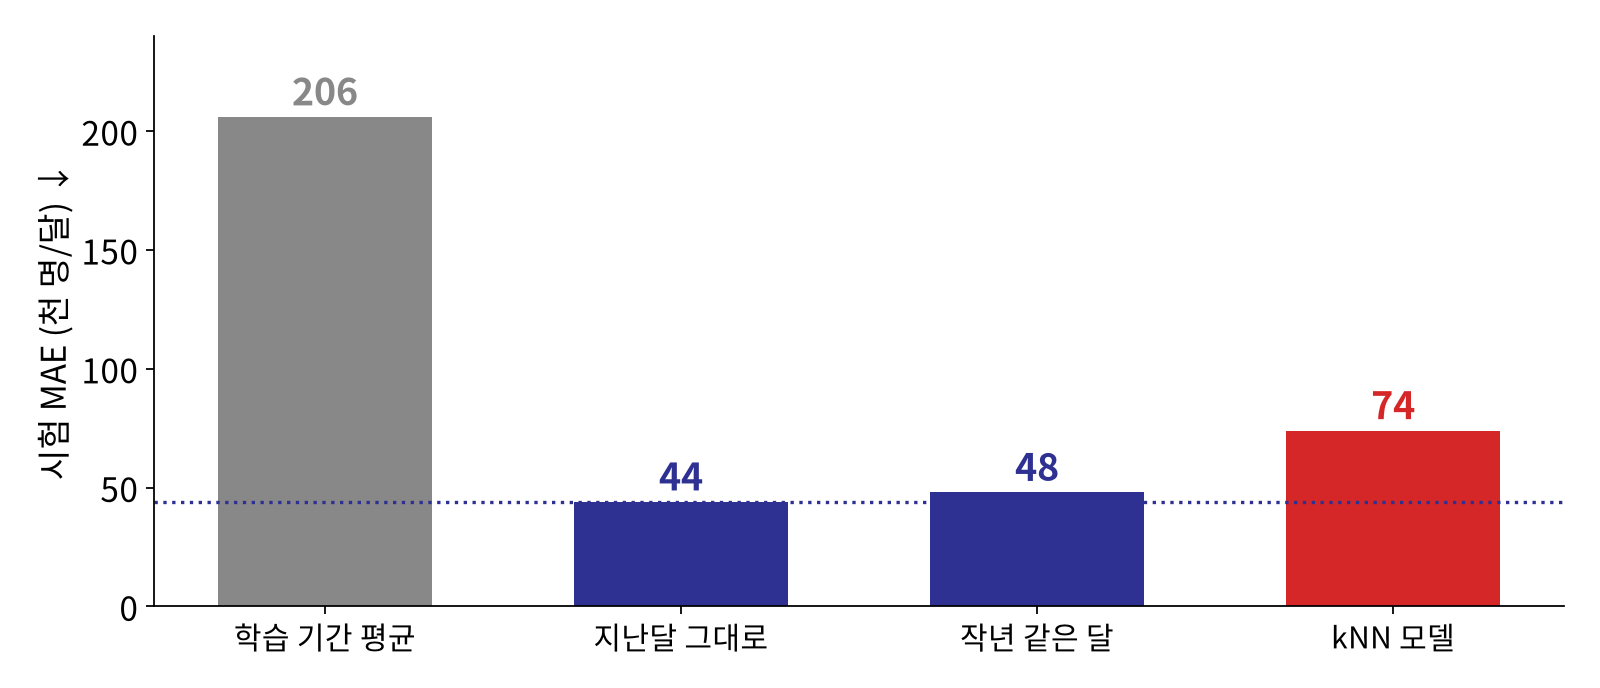
\includegraphics[width=0.72\linewidth]{pf_air.png}\par\vskip0.3em
{\large 지난 12달을 보고 고른 kNN 모델 \kq{74}, ``지난달 그대로'' \kb{44}천 명}\\[0.3em]
{\scriptsize 국제선 항공 승객 1949$\sim$1960, 앞 10년 학습 · 뒤 2년 (24달) 시험, MAE (천 명/달). kNN: $k = 3$, 학습 기간 평균 · 표준편차로 표준화}
\vfill
\note{항공 승객의 다음 달을 예측합니다. 회색은 늘 학습 기간 평균이라고 답한 것, 206천 명이나 틀립니다. 파란 두 막대가 기준선, 지난달 그대로와 작년 같은 달입니다. 44와 48. 그리고 빨간 막대가 지난 12달 패턴을 보고 비슷한 과거를 찾아오는 kNN 모델, 74입니다. 모델이 지난달 값을 그대로 적는 것보다 못합니다. 기준선을 안 재 봤다면 이걸 몰랐을 겁니다. 다음 시간에 정규화를 창마다 하면 이 모델이 10까지 내려가는 걸 봅니다.}
\end{frame}

% --- 시험은 미래
\begin{frame}{시험 데이터 = 모델이 ``실제로 만날'' 데이터}
\vfill
\centering
{\large
\begin{tabular}{ll}
\textbf{데이터} & \textbf{어떻게 나누나}\\[0.2em]\hline\\[-0.6em]
와인 178병 & 무작위로 70\% 학습 · 30\% 시험 (품종 비율은 맞춰서)\\[0.5em]
항공 승객 & \kb{시간 순서대로}: 1949$\sim$1958 학습, 1959$\sim$1960 시험\\[0.5em]
은행 거래 & \kb{시간 순서대로}: 앞 기간으로 학습, 뒤 기간으로 시험\\[0.5em]
영화 별점 & 가장 최근 별점을 \kb{숨겨서} 시험 (넷플릭스 프라이즈)
\end{tabular}}\vskip1.2em
{\large 미래를 섞어 학습하면 \kq{시험 점수가 거짓말}을 한다}
\vfill
\note{평가지표만큼 중요한 게 어떤 데이터로 채점하느냐입니다. 시험 데이터는 모델이 실제로 쓰일 때 만날 데이터를 흉내 내야 합니다. 와인처럼 순서가 없으면 무작위로 나눠도 됩니다. 하지만 승객 수나 은행 거래는 미래를 예측하는 게 목적이니 시간 순서대로, 과거로 학습하고 미래로 시험합니다. 무작위로 섞으면 내일 값을 보고 오늘을 맞히는 셈이 되어 시험 점수가 실제보다 좋게 나옵니다. 넷플릭스 프라이즈는 아예 가장 최근 별점을 숨겨 두고 그걸로 시험했습니다. 이건 뒤에서 봅니다.}
\end{frame}

% --- AML 열어 보기
\begin{frame}{자금세탁 데이터 열어 보기: 한 행 = 거래 한 건}
\vfill
\centering
{\scriptsize\setlength{\tabcolsep}{3.5pt}
\begin{tabular}{lllrlll}
\textbf{Timestamp} & \textbf{From (은행, 계좌)} & \textbf{To (은행, 계좌)} & \textbf{Amount Paid} & \textbf{Currency} & \textbf{Format} & \textbf{Is Laundering}\\\hline
\amlRowA\\
\amlRowB\\
\multicolumn{7}{c}{$\vdots$}
\end{tabular}}\vskip1em
{\large 거래 \amlN 건, 그중 세탁 \kq{\amlPos 건 (\amlRate\%)}}\vskip0.6em
{\normalsize 입력 $X$: 시각 · 보낸 쪽 · 받는 쪽 · 금액 · 통화 · 결제 형식 \qquad 출력 $y$: \texttt{Is Laundering} (0/1)}\\[0.4em]
{\scriptsize IBM 이 가상 세계(사람 · 회사 · 은행)를 시뮬레이션해 만든 합성 데이터 (Altman et al., NeurIPS 2023). 실제 은행 거래는 공개할 수 없어서 이렇게 만든다}
\vfill
\note{이제 자금세탁 데이터를 열어 봅니다. IBM이 사람, 회사, 은행이 있는 가상 세계를 시뮬레이션해 만든 합성 데이터입니다. 실제 은행 거래는 개인정보라 공개할 수 없어서, 세탁 수법까지 흉내 낸 가짜 세계를 만든 겁니다. 한 행이 거래 한 건입니다. 시각, 보낸 은행과 계좌, 받는 은행과 계좌, 금액, 통화, 결제 형식, 그리고 정답 칸 Is Laundering. 거래가 \amlN 건인데 세탁은 \amlPos 건, \amlRate 퍼센트입니다. 표는 파일의 실제 첫 두 줄입니다.}
\end{frame}

% --- 정확도의 함정
\begin{frame}{정확도의 함정: 드문 것을 찾는 문제}
\vfill
\centering
{\large
\begin{tabular}{lcc}
& \textbf{전부 ``정상''} & \textbf{규칙: 결제 형식이 \amlFmt 면 ``세탁''}\\[0.2em]\hline\\[-0.6em]
정확도 & \kq{\amlAccZero\%} & \amlAccRule\%\\[0.5em]
잡아낸 세탁 거래 & \kq{0 건} & \kb{\amlTP 건}
\end{tabular}}\vskip1.4em
{\large 세탁을 \kq{하나도 못 잡는} 쪽이 정확도는 더 높다}\vskip0.6em
{\small 세탁이 드물어서, ``정상''을 맞힌 수가 점수를 거의 다 차지한다}
\vfill
\note{두 모델을 비교해 봅시다. 왼쪽은 전부 정상이라고 답합니다. 정확도 \amlAccZero 퍼센트, 잡아낸 세탁은 0건. 오른쪽은 아주 단순한 규칙 하나, 세탁 비율이 가장 높은 결제 형식 \amlFmt 이면 세탁이라고 답합니다. 정확도는 \amlAccRule 퍼센트로 오히려 낮은데, 세탁 \amlTP 건을 잡아냅니다. 드문 것을 찾는 문제에서 정확도는 거의 정상을 맞힌 수로만 정해지기 때문에, 우리가 원하는 걸 재지 못합니다.}
\end{frame}

% --- 세는 법을 바꾼다
\begin{frame}{그래서 세는 법을 바꾼다: 정밀도와 재현율}
\vfill
\centering
{\large
\begin{tabular}{l|cc}
& \textbf{실제 세탁} & \textbf{실제 정상}\\\hline
\textbf{``세탁''이라고 함} & \kb{\amlTP} (잡았다) & \kq{\amlFP} (헛짚었다)\\
\textbf{``정상''이라고 함} & \kq{\amlFN} (놓쳤다) & (나머지)
\end{tabular}}\vskip1.2em
{\large 재현율 (recall) $= \dfrac{\text{잡았다}}{\text{실제 세탁 전부}} = \dfrac{\amlTP}{\amlTP + \amlFN} = \kb{\amlRec\%}$}\vskip0.6em
{\large 정밀도 (precision) $= \dfrac{\text{잡았다}}{\text{``세탁''이라고 한 것 전부}} = \dfrac{\amlTP}{\amlTP + \amlFP} = \kq{\amlPrec\%}$}\vskip0.8em
{\small 전부 ``정상''은 재현율 0\%. 자세한 계산과 둘 사이의 줄다리기는 2주차 (정밀도와 재현율)}
\vfill
\note{그래서 세는 법을 바꿉니다. 실제 세탁 거래 중에서 몇 개를 잡았나, 이게 재현율입니다. 규칙은 \amlRec 퍼센트, 꽤 많이 잡습니다. 세탁이라고 찍은 것 중에 진짜 세탁이 몇 개였나, 이게 정밀도입니다. \amlPrec 퍼센트. 세탁이라고 찍은 60만 건 중 진짜는 4천 5백 건뿐이라, 이 규칙대로 조사하면 헛걸음이 대부분입니다. 전부 정상이라고 하는 모델은 재현율이 0입니다. 정확도 \amlAccZero 퍼센트에 가려 있던 사실이 드러납니다. 이 두 지표는 2주차에 자세히 다룹니다. 오늘은 무엇을 세느냐가 점수의 의미를 바꾼다는 것만 기억하세요.}
\end{frame}

% --- 한 행을 무엇으로
\begin{frame}{한 행을 무엇으로 정하나: 거래 vs 계좌}
\vfill
\centering
{\large
\begin{tabular}{lll}
& \textbf{한 행 = 거래 한 건} & \textbf{한 행 = 보낸 계좌 하나}\\[0.2em]\hline\\[-0.6em]
행 수 & \amlN & \amlAcct\\[0.4em]
$y = 1$ 인 행 & \amlPos & \amlAcctPos\\[0.4em]
세탁 비율 & \kq{\amlRate\%} & \kb{\amlAcctRate\%}\\[0.4em]
현실의 질문 & 이 송금을 막을까? & 이 계좌를 조사할까?
\end{tabular}}\vskip1.2em
{\large 같은 파일, 다른 문제. 논문마다 ``세탁 비율''이 다르게 적힌 이유}
\vfill
\note{다섯 칸의 첫 칸, 한 행을 무엇으로 정하느냐도 문제를 바꿉니다. 거래 한 건을 한 행으로 보면 세탁 비율은 \amlRate 퍼센트입니다. 그런데 은행이 실제로 하는 일은 거래 하나하나를 막기보다 수상한 계좌를 조사하는 겁니다. 계좌 하나를 한 행으로, 세탁 거래를 한 번이라도 보냈으면 1로 정하면 행 수는 \amlAcct, 비율은 \amlAcctRate 퍼센트가 됩니다. 같은 파일인데 다른 문제입니다. 실제로 이 데이터를 쓴 논문들을 보면 세탁 비율이 서로 다르게 적혀 있는데, 이렇게 한 행을 다르게 정했기 때문입니다.}
\end{frame}

% --- 넷플릭스 프라이즈
\begin{frame}{문제를 먼저 공개한 대회: 넷플릭스 프라이즈 (2006)}
\markpage{netflix}
\vfill
\centering
{\large
\begin{tabular}{rl}
\textbf{한 행} & (사용자, 영화, 날짜) 하나\\[0.45em]
\textbf{입력 $X$} & 사용자 번호 · 영화 번호 · 날짜\\[0.45em]
\textbf{출력 $y$} & 별점 1 $\sim$ 5\\[0.45em]
\textbf{평가지표} & \kb{RMSE} (별 몇 개만큼 틀리나)\\[0.45em]
\textbf{기준선} & 넷플릭스의 추천 시스템 Cinematch: RMSE \kq{0.95}\\[0.45em]
\textbf{목표} & 그보다 \kq{10\%} 나은 팀에게 상금 \kb{100만 달러}
\end{tabular}}\vskip1em
{\small 공개한 데이터: 사용자 48만 명 이상 · 영화 약 1만 8천 편 · 별점 1억 개 이상 (1998 $\sim$ 2005)}
\vfill
\note{2006년 넷플릭스는 자기 추천 시스템보다 10퍼센트 나은 팀에게 100만 달러를 주겠다고 했습니다. 다섯 칸이 처음부터 공개됐습니다. 한 행은 사용자, 영화, 날짜 하나. 출력은 별점 1에서 5. 채점은 RMSE, 별 몇 개만큼 틀리나. 기준선은 넷플릭스가 쓰던 Cinematch, RMSE 약 0.95. 이보다 10퍼센트 나으면 우승입니다. 사용자 48만 명이 영화 약 1만 8천 편에 남긴 별점 1억 개를 공개했습니다.}
\end{frame}

% --- 숨긴 시험
\begin{frame}{시험 데이터를 \textbf{숨겼다}: 가장 최근 별점 300만 개}
\vfill
\centering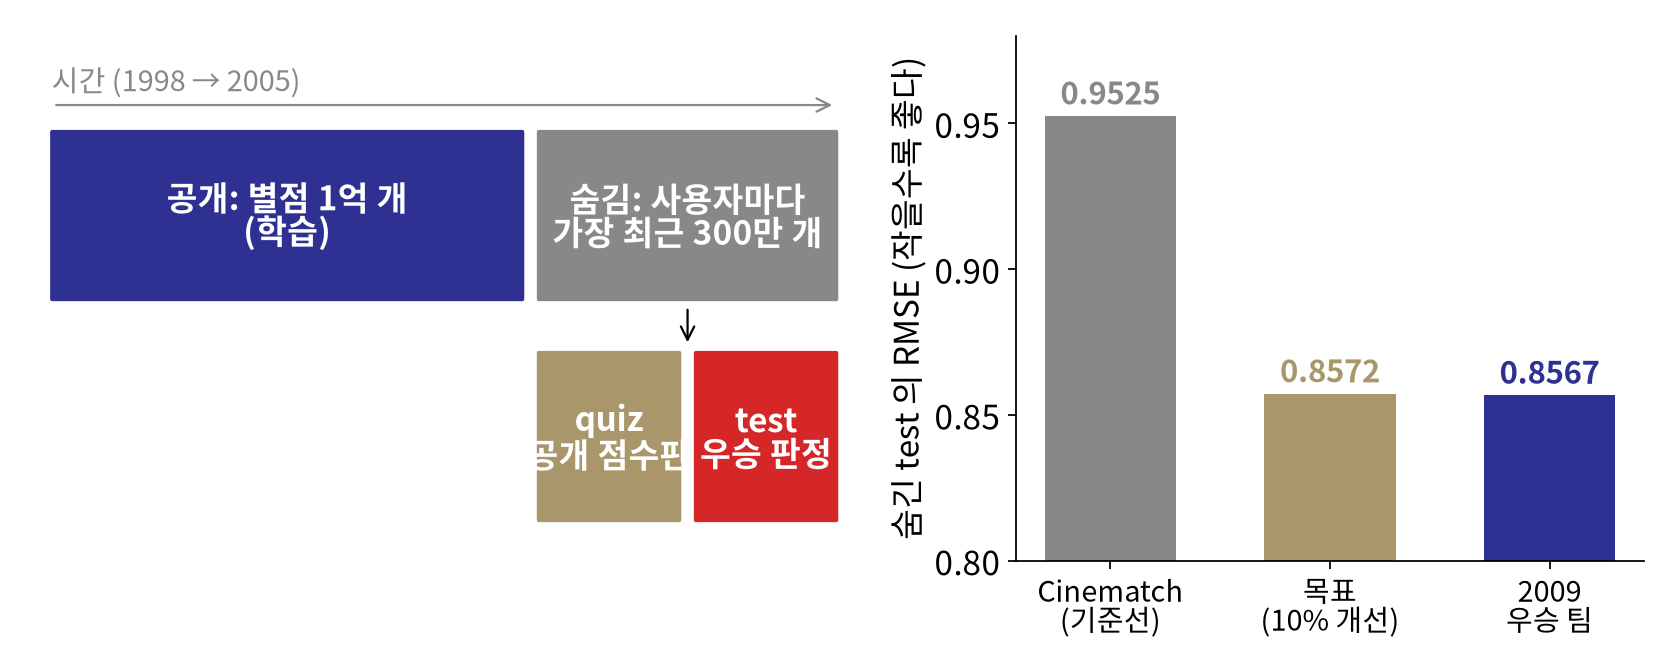
\includegraphics[width=0.86\linewidth]{pf_netflix.png}\par\vskip0.3em
{\large 공개 점수판은 숨긴 별점의 \kb{절반 (quiz)} 으로만. 우승은 \kq{나머지 절반 (test)} 으로 판정}\\[0.3em]
{\small 점수판에 맞춰 계속 고치면 점수판에만 잘 맞는 모델이 된다 (과대적합, 2주차)}
\vfill
\note{채점 방식이 정교했습니다. 사용자마다 가장 최근 별점을 숨겼습니다. 미래를 맞히는 문제니까 시간 순서로 나눈 겁니다. 숨긴 별점 300만 개 중 절반은 제출할 때마다 점수를 알려 주는 공개 점수판에 쓰고, 나머지 절반은 아무도 점수를 모르게 두었다가 우승을 판정할 때만 썼습니다. 점수판을 보면서 계속 고치면 점수판에만 잘 맞는 모델이 되기 때문입니다. 숨긴 시험에서 Cinematch 는 0.9525, 10퍼센트 나은 목표는 0.8572였습니다. 2009년, 3년 만에 BellKor's Pragmatic Chaos 팀이 0.8567로 목표를 넘겨 우승했습니다. 같은 점수를 낸 다른 팀은 20분 늦게 제출해서 졌습니다.}
\end{frame}

% --- 그 뒤
\begin{frame}{우승한 모델, 그런데 그대로 쓰지는 않았다}
\vfill
\centering
{\large
\begin{tabular}{ll}
\textbf{2009} & 우승 팀: 100개가 넘는 모델을 섞은 앙상블, RMSE \kb{0.8567}\\[0.5em]
\textbf{그 뒤} & 넷플릭스는 대회 중간 (2007) 에 나온 방법 두 가지만 가져다 썼다\\
& 최종 앙상블은 \kq{들일 품에 비해 좋아지는 게 작았다}\\[0.5em]
\textbf{그 사이} & DVD 대여 $\to$ 스트리밍: '별점' 보다 '무엇을 끝까지 보나' 가 중요해졌다
\end{tabular}}\vskip1.2em
{\large 지표 (RMSE) 를 이기는 것과 \kq{사업이 좋아지는 것}은 다르다}
\vfill
\note{우승 모델은 100개가 넘는 모델을 섞은 거대한 앙상블이었습니다. 넷플릭스는 대회 중간에 나온 좋은 방법 몇 가지는 실제로 가져다 썼지만, 최종 우승 모델 전체는 쓰지 않았습니다. 마지막 몇 퍼센트를 위해 들어가는 엔지니어링 품이 너무 컸기 때문입니다. 그 사이 회사도 DVD 대여에서 스트리밍으로 바뀌어서, 별점을 맞히는 것보다 사람들이 무엇을 끝까지 보는지가 더 중요해졌습니다. 지표를 이기는 것과 사업이 좋아지는 것은 다를 수 있습니다. 다음 장이 그 이야기입니다.}
\end{frame}

% --- 지표만 쫓는다
\begin{frame}{지표를 정하면, 모델은 그 지표만 쫓는다}
\vfill
\centering
{\large
\begin{tabular}{ll}
\textbf{지표} & \textbf{이 점수를 최대로 만드는 가장 쉬운 방법}\\[0.2em]\hline\\[-0.6em]
정확도 & 전부 ``정상'' $\to$ \amlAccZero\%\\[0.5em]
재현율 & 전부 ``세탁'' $\to$ 100\% (그런데 은행이 멈춘다)\\[0.5em]
정밀도 & 가장 확실한 한 건만 ``세탁'' $\to$ 100\% (나머지는 다 놓친다)
\end{tabular}}\vskip1.4em
{\large 지표는 \kq{현실에서 무엇이 손해인지}에서 거꾸로 정한다}\\[0.4em]
{\small 놓친 세탁 한 건의 손해 vs 헛짚어 정상 고객을 막은 한 건의 손해}
\vfill
\note{지표를 하나 정하면 모델은 그 점수만 올리려고 합니다. 정확도만 보면 전부 정상, 재현율만 보면 전부 세탁이라고 하면 100퍼센트입니다. 대신 모든 송금이 막혀 은행이 멈추겠죠. 정밀도만 보면 가장 확실한 한 건만 세탁이라고 하면 됩니다. 그래서 지표는 현실에서 무엇이 손해인지에서 거꾸로 정해야 합니다. 세탁 한 건을 놓치는 손해와, 정상 고객 한 명을 잘못 막는 손해 중 무엇이 더 큰가. 이건 수학이 아니라 그 분야의 판단입니다.}
\end{frame}

% --- 문제풀이
\begin{frame}{문제풀이}
\vfill
\begin{enumerate}
\item 다섯 칸을 채워 보자: \quad (a) 스팸 문자 거르기 \quad (b) 내일 서울 최고 기온 \quad (c) 사진 속 고양이 위치 찾기\vskip0.6em
\item 예측 \texttt{[10, 20, 30, 40]}, 정답 \texttt{[12, 18, 30, 50]}. MAE 와 RMSE 는?\vskip0.6em
\item 환자 1,000명 중 20명이 병에 걸렸다. ``전부 건강''의 정확도는? 재현율은?\vskip0.6em
\item 내일 주가를 맞히는 모델의 입력에 ``내일 거래량''을 넣었더니 성능이 크게 올랐다. 무엇이 잘못됐나?\vskip0.6em
\item 학생 성적 데이터에서 시험 데이터를 무작위로 뽑았는데, 같은 학생의 다른 학기 기록이 학습 데이터에 있다. 무엇이 문제일까?
\end{enumerate}
\vfill
\note{1번 예시 답. 스팸은 한 행이 문자 하나, 입력은 문자 내용, 출력은 스팸이냐 아니냐, 지표는 스팸이 드물면 정밀도와 재현율, 기준선은 전부 정상. 기온은 한 행이 하루, 입력은 오늘까지의 날씨, 출력은 내일 최고 기온, 지표는 MAE, 기준선은 오늘 기온 그대로. 고양이 위치는 한 행이 사진 하나, 출력은 상자 좌표 네 개, 지표는 상자가 겹치는 정도. 2번. 오차가 2, 2, 0, 10이라 MAE는 14 나누기 4, 3.5. RMSE는 4 더하기 4 더하기 0 더하기 100, 108 나누기 4는 27, 루트 27은 약 5.2. 3번. 정확도 98퍼센트, 재현율 0퍼센트. 4번. 내일 거래량은 오늘 예측할 때 알 수 없는 값입니다. 입력에는 예측하는 순간 알 수 있는 것만 넣어야 합니다. 5번. 같은 학생이 학습과 시험 양쪽에 있으면 모델이 학생을 외워서 맞힙니다. 새 학생에게 쓸 모델이라면 학생 단위로 나눠야 합니다.}
\end{frame}

% --- 실습
\begin{frame}[fragile]{실습: 문제를 직접 정해 보기}
\vfill
\centering\begin{tabular}{rl}
\large 1 & 와인: 같은 데이터로 분류 · 회귀 두 문제 만들기, 정확도 · MAE · 기준선 직접 구현\\[0.4em]
\large 2 & 항공 승객: 지난달 그대로 · 작년 같은 달 vs kNN (\kq{74} vs \kb{44})\\[0.4em]
\large 3 & IBM AML: 거래 \amlN 건 열기, 전부 ``정상'' \amlAccZero\%, 규칙 하나의 정밀도 · 재현율,\\
& 한 행을 계좌로 바꾸면 (\amlRate\% $\to$ \amlAcctRate\%)\\[0.4em]
\large 4 & 넷플릭스 프라이즈 축소판: MovieLens 별점, 사람마다 최근 별점을 숨겨 RMSE · 10\% 개선 목표
\end{tabular}\vskip0.8em
AML 은 Hugging Face 사본에서 받는다 (로그인 없이, 압축 약 90MB) \\[0.3em]\href{https://colab.research.google.com/github/SuminHan/book-ml/blob/main/slides/v2/ml1/week01/problem_formulation/lab/problem_formulation.ipynb}{\textcolor{ksagolddk}{▶ Colab에서 실습 노트북 열기}}
\vfill
\note{실습에서는 네 가지 데이터로 직접 다섯 칸을 채웁니다. 와인으로 분류와 회귀 두 문제를 만들고, 정확도, MAE, 기준선을 직접 함수로 만듭니다. 항공 승객에서는 기준선이 모델을 이기는 걸 확인합니다. 자금세탁 데이터는 파일이 커서 처음 받을 때 몇 분 걸립니다. 마지막으로 넷플릭스 프라이즈를 작게 따라 해 봅니다. 영화 별점에서 사람마다 가장 최근 별점을 숨기고, 기준선보다 10퍼센트 나아지는지 봅니다.}
\end{frame}

% --- 정리
\begin{frame}{정리}
\vfill
\centering\large\begin{tabular}{l}
문제 = \kb{다섯 칸}: 한 행 · 입력 $X$ · 출력 $y$ · 평가지표 · 기준선\\[0.45em]
같은 데이터라도 $y$ 와 \kb{한 행}을 다르게 정하면 다른 문제 (와인, 거래 vs 계좌)\\[0.45em]
점수는 \kq{기준선과 비교}해서 읽는다 (모델이 ``지난달 그대로''에 질 수도)\\[0.45em]
시험 데이터는 실제로 만날 데이터처럼: 시간 순서, 사람 · 지역 단위\\[0.45em]
지표는 현실의 손해에서 거꾸로 정한다. 시험 데이터는 \kb{숨긴다} (넷플릭스 프라이즈)
\end{tabular}
\vfill
\note{정리합니다. 머신러닝 문제는 다섯 칸, 한 행, 입력, 출력, 평가지표, 기준선입니다. 같은 데이터라도 y와 한 행을 다르게 정하면 다른 문제가 됩니다. 점수는 반드시 기준선과 비교해서 읽습니다. 시험 데이터는 모델이 실제로 만날 데이터처럼 나눕니다. 지표는 현실에서 무엇이 손해인지에서 거꾸로 정합니다. 넷플릭스 프라이즈처럼 문제와 지표와 숨긴 시험이 먼저 단단히 정해져 있어야, 누가 더 잘했는지 모두가 받아들일 수 있습니다. 다음 시간에는 데이터를 직접 열어 청소하고 정규화합니다.}
\end{frame}

% --- 출처
\begin{frame}{이미지 · 데이터 출처}
\vfill
\small
\begin{itemize}
\item 자금세탁 거래: IBM Transactions for Anti Money Laundering (HI-Small), Kaggle \texttt{ealtman2019} (실습은 Hugging Face 사본); Altman et al., ``Realistic Synthetic Financial Transactions for Anti-Money Laundering Models'' (NeurIPS 2023 Datasets and Benchmarks)
\item 넷플릭스 프라이즈: Bennett \& Lanning (2007) ``The Netflix Prize'', KDD Cup and Workshop; 우승 결과 (2009) 와 이후 사용은 넷플릭스 기술 블로그 (2012)
\item 와인: UCI Wine (Aeberhard \& Forina, 1991) \quad 항공 승객: Box \& Jenkins, \textit{Time Series Analysis} (1976)
\end{itemize}
\vfill
\note{이 덱에 쓴 데이터의 출처입니다.}
\end{frame}
\end{document}
